% Options for packages loaded elsewhere
\PassOptionsToPackage{unicode}{hyperref}
\PassOptionsToPackage{hyphens}{url}
%
\documentclass[
]{book}
\usepackage{amsmath,amssymb}
\usepackage{iftex}
\ifPDFTeX
  \usepackage[T1]{fontenc}
  \usepackage[utf8]{inputenc}
  \usepackage{textcomp} % provide euro and other symbols
\else % if luatex or xetex
  \usepackage{unicode-math} % this also loads fontspec
  \defaultfontfeatures{Scale=MatchLowercase}
  \defaultfontfeatures[\rmfamily]{Ligatures=TeX,Scale=1}
\fi
\usepackage{lmodern}
\ifPDFTeX\else
  % xetex/luatex font selection
\fi
% Use upquote if available, for straight quotes in verbatim environments
\IfFileExists{upquote.sty}{\usepackage{upquote}}{}
\IfFileExists{microtype.sty}{% use microtype if available
  \usepackage[]{microtype}
  \UseMicrotypeSet[protrusion]{basicmath} % disable protrusion for tt fonts
}{}
\makeatletter
\@ifundefined{KOMAClassName}{% if non-KOMA class
  \IfFileExists{parskip.sty}{%
    \usepackage{parskip}
  }{% else
    \setlength{\parindent}{0pt}
    \setlength{\parskip}{6pt plus 2pt minus 1pt}}
}{% if KOMA class
  \KOMAoptions{parskip=half}}
\makeatother
\usepackage{xcolor}
\usepackage{longtable,booktabs,array}
\usepackage{calc} % for calculating minipage widths
% Correct order of tables after \paragraph or \subparagraph
\usepackage{etoolbox}
\makeatletter
\patchcmd\longtable{\par}{\if@noskipsec\mbox{}\fi\par}{}{}
\makeatother
% Allow footnotes in longtable head/foot
\IfFileExists{footnotehyper.sty}{\usepackage{footnotehyper}}{\usepackage{footnote}}
\makesavenoteenv{longtable}
\usepackage{graphicx}
\makeatletter
\def\maxwidth{\ifdim\Gin@nat@width>\linewidth\linewidth\else\Gin@nat@width\fi}
\def\maxheight{\ifdim\Gin@nat@height>\textheight\textheight\else\Gin@nat@height\fi}
\makeatother
% Scale images if necessary, so that they will not overflow the page
% margins by default, and it is still possible to overwrite the defaults
% using explicit options in \includegraphics[width, height, ...]{}
\setkeys{Gin}{width=\maxwidth,height=\maxheight,keepaspectratio}
% Set default figure placement to htbp
\makeatletter
\def\fps@figure{htbp}
\makeatother
\setlength{\emergencystretch}{3em} % prevent overfull lines
\providecommand{\tightlist}{%
  \setlength{\itemsep}{0pt}\setlength{\parskip}{0pt}}
\setcounter{secnumdepth}{5}
\usepackage{booktabs}
\ifLuaTeX
  \usepackage{selnolig}  % disable illegal ligatures
\fi
\usepackage[]{natbib}
\bibliographystyle{plainnat}
\usepackage{bookmark}
\IfFileExists{xurl.sty}{\usepackage{xurl}}{} % add URL line breaks if available
\urlstyle{same}
\hypersetup{
  pdftitle={6ª EcoEscola: livro de resumos},
  pdfauthor={Gabriel Nakamura},
  hidelinks,
  pdfcreator={LaTeX via pandoc}}

\title{6ª EcoEscola: livro de resumos}
\author{Gabriel Nakamura}
\date{2025-03-26}

\begin{document}
\maketitle

{
\setcounter{tocdepth}{1}
\tableofcontents
}
\chapter{Sobre}\label{sobre}

Este livro contém os resumos dos projetos realizados durante a 6ª EcoEscola

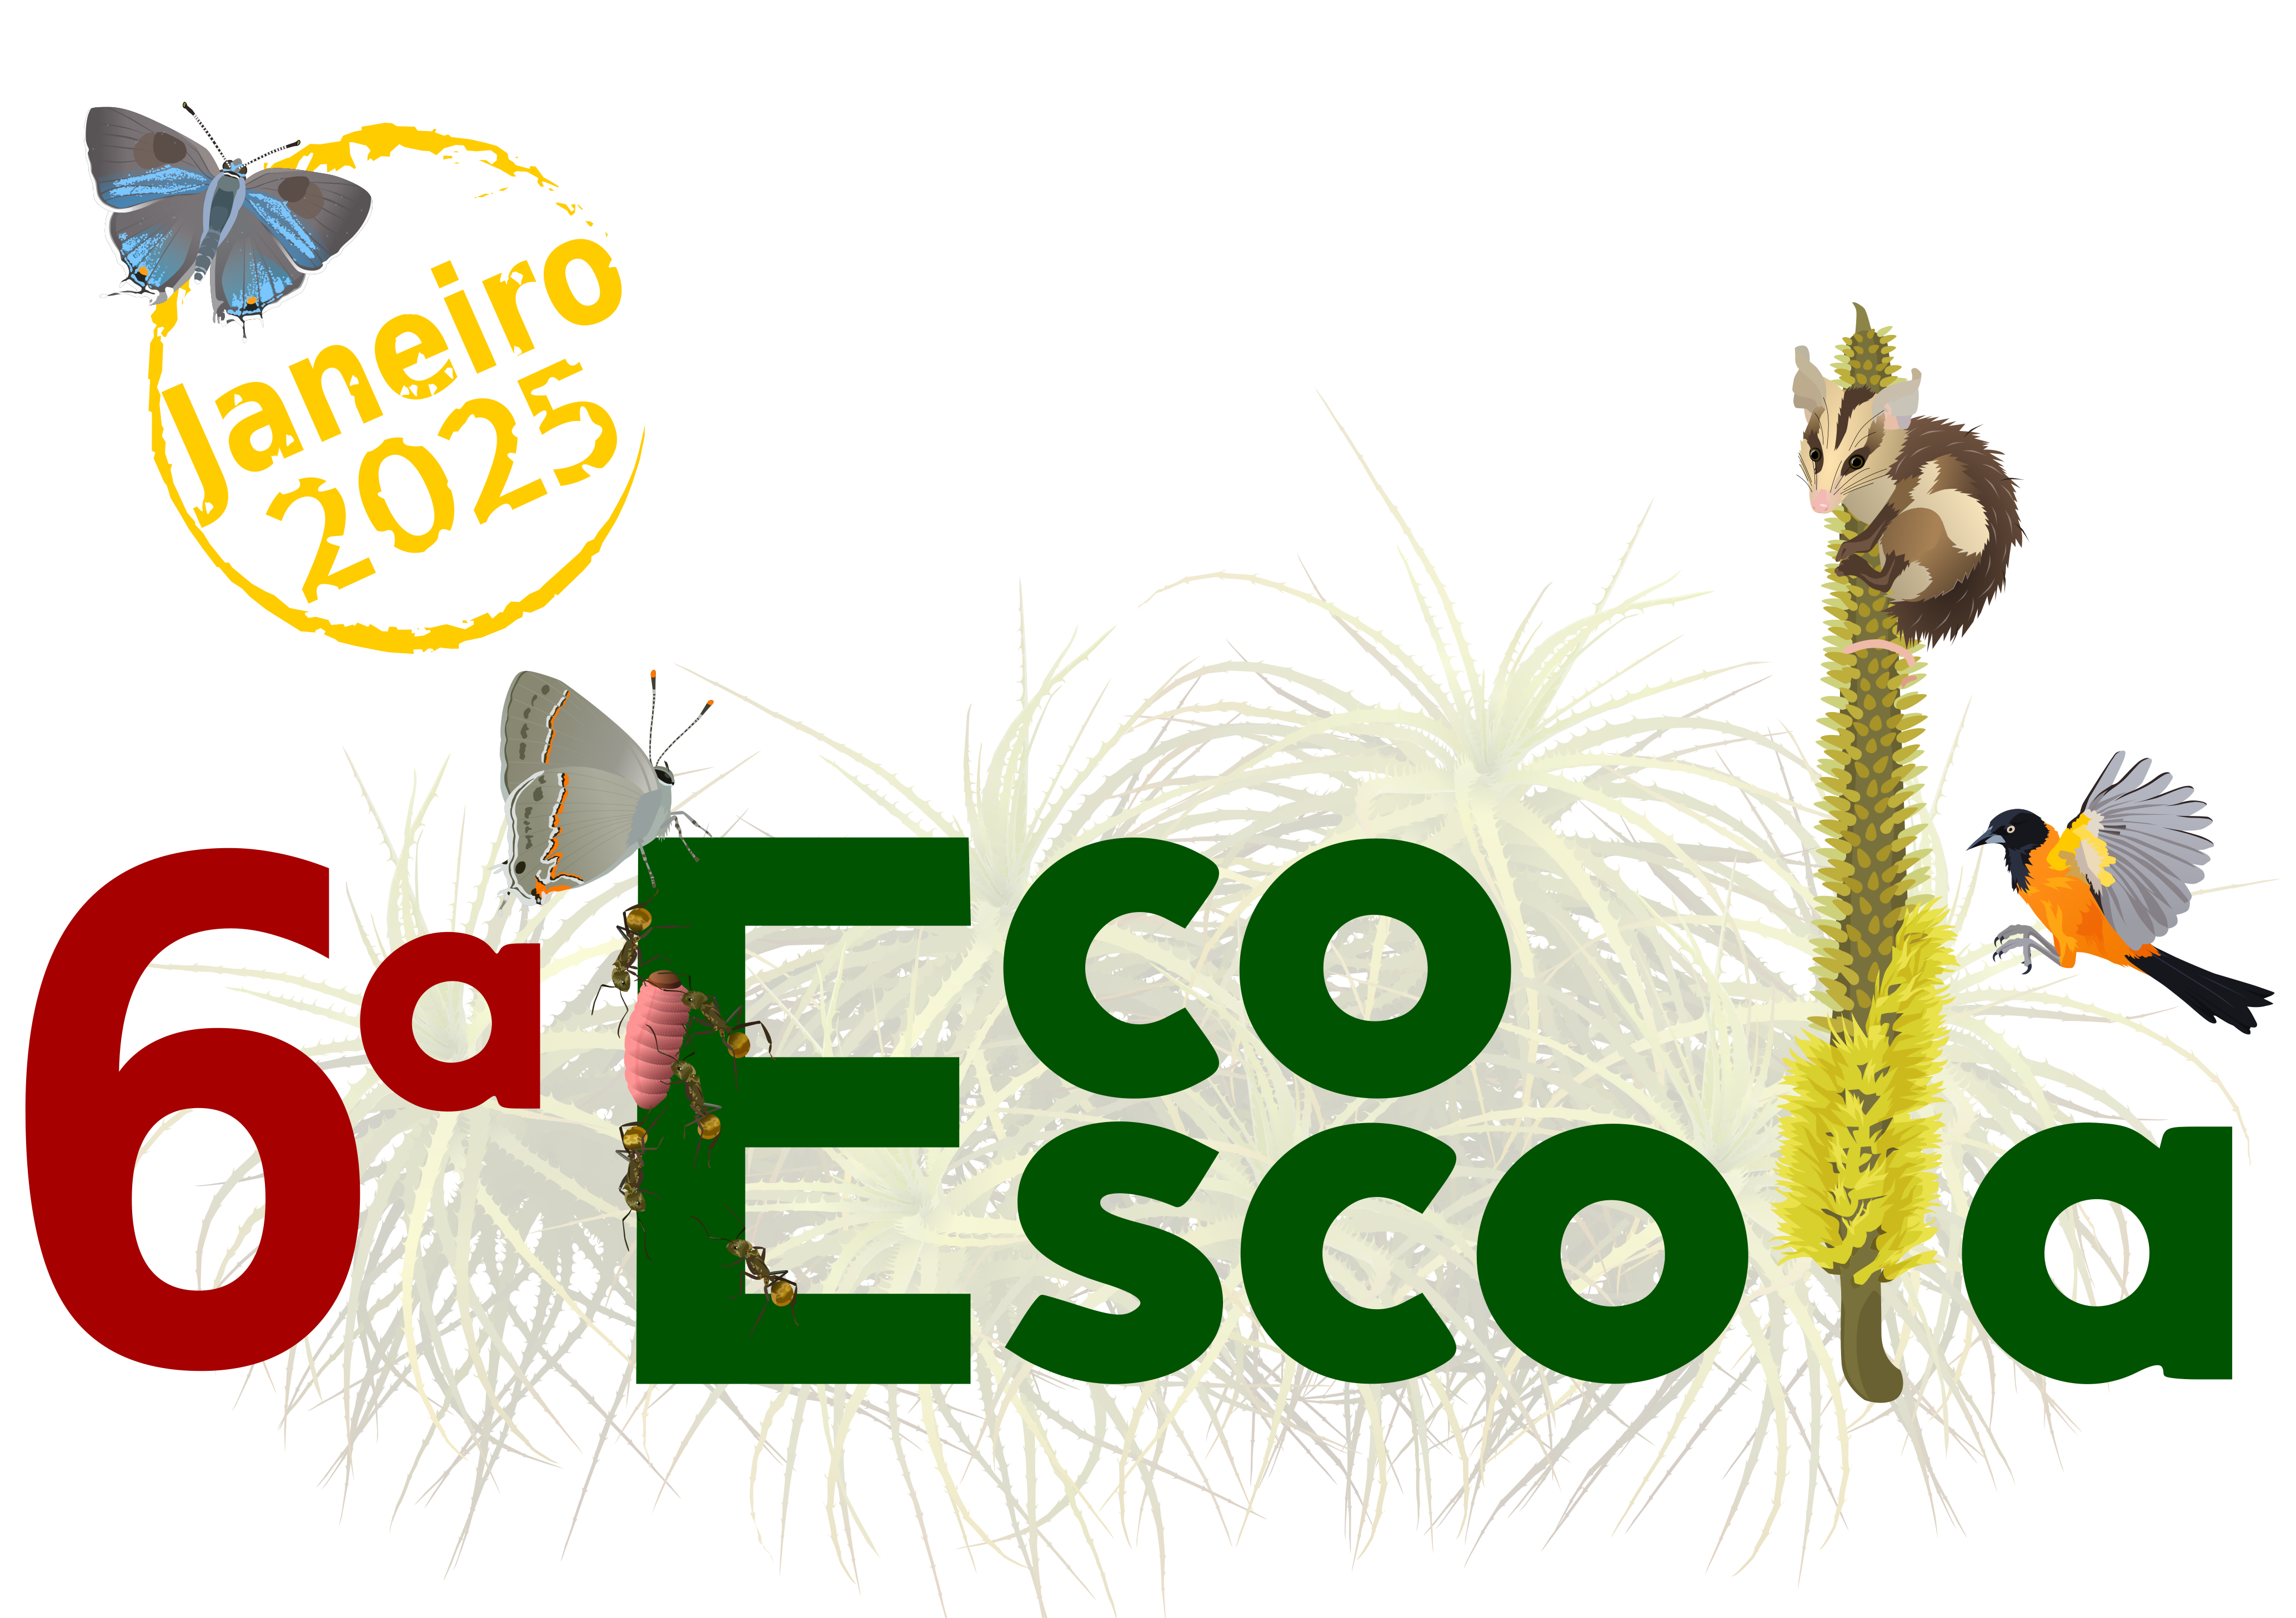
\includegraphics{figs/ecoescolalogo.png}

\chapter{Introdução}\label{introduuxe7uxe3o}

Este livro contém os resumos dos trabalhos realizados durante a 6ª EcoEscola.
Esta é a primeira iniciativa de organização dos resumos. Pretendemos que este
material sirva de duas formas. Para apresentar os projetos realizados durante
o módulo prático da EcoEscola, e que sirva como fonte de inspiração para projetos
rápidos (duas semanas) que envolvam coleta, análise e interpretação de dados.
Pretendemos que este material também sirva para professores e educadores de
ensino superior e médio para fornecer possíveis atividades práticas que possam
ser utilizadas em aulas de ensino de Ecologia para nível médio e superior.

\section{A EcoEscola}\label{a-ecoescola}

Descrever o que é a ecoescola

\section{Ensino por investigação}\label{ensino-por-investigauxe7uxe3o}

\section{Os projetos}\label{os-projetos}

\chapter{\texorpdfstring{Cobertura e dominância de samambaias epífitas em \emph{Tipuana tipu}}{Cobertura e dominância de samambaias epífitas em Tipuana tipu}}\label{cobertura-e-dominuxe2ncia-de-samambaias-epuxedfitas-em-tipuana-tipu}

\begin{quote}
Grupo 1: Francelino, A.C., Ribeiro, C.F.F., Santos, G.P., Batista, L.R.C., Bergmann, M.A.~e Cirino, D.W.
\end{quote}

\begin{quote}
Orientador: Douglas William Cirino
\end{quote}

Plantas pteridófitas utilizam árvores como forófitos, representando uma interação interespecífica neutra, onde não há prejuízos à planta hospedeira. Nessa interação, o espaço nos galhos do forófito é um importante recurso, gerando competição entre epífitas, com cenários de dominância ou coexistência, a depender do ambiente. O objetivo deste trabalho foi compreender se há relação dos microclimas com a cobertura e a coexistência de pteridófitas epífitas no forófito Tipuana tipu (Benth.) Kuntze. Nossa hipótese é que a dominância da epífita Microgramma sp. em relação a outras pteridófitas é menor em cenários de microclima mais favorável. Além disso, supomos que quanto maior o índice de vegetação maior será a cobertura vegetal total de epífitas nos galhos de Tipuana tipu. Amostramos 40 indivíduos do forófito sob diferentes condições microclimáticas.. Fotografamos quadrantes de 50x50 cm, a diferentes alturas na face sul de cada Tipuana tipu (Benth.) Kuntze. Estimamos as áreas de cobertura de três morfotipos de pteridófitas mais comuns. Calculamos a dominância de Microgramma sp. sobre outras epífitas como uma proporção da área total coberta por (NDVI) utilizando ortofotos de 1m de resolução e medimos o NDVI médio dentro de buffers de 25, 50 e 100m de raio a partir do forófito. Testamos nossas hipóteses utilizando a função betareg do software R (V 4.4.2). Nosso resultado demonstra que quanto maior a média do NDVI nos buffers de 25 e 50m menor será a dominância da Microgramma sp. (p=0,010 e p=0,026, respectivamente), corroborando nossa hipótese, enquanto não houve diferença estatística no buffer de 100m (p=0,153). Adicionalmente, não houve relação estatística entre o NDVI e a cobertura das epífitas (p\textgreater0,05). Isso pode indicar que o microclima pode não ser o fator principal influenciando essa ocupação, refutando nossa segunda hipótese. Por outro lado, pudemos confirmar que o microclima é preponderante na dominância de Microgramma sp. sobre as outras samambaias epífitas, uma vez que em raios menores o efeito é significativo e em raios de 100m o efeito desaparece. Estudos anteriores afirmam que a interação entre epífitas com diferentes formas de dispersão pode ser negativa1, Microgramma sp. é a única epífita trepadeira amostrada, podendo ser dominante, mas em microclimas mais favoráveis a competição pode ser mais intensa.. Como hipótese a posteriori, corroboramos que quanto maior a altura da amostra no forófito maior será a cobertura de epífitas (p=0,001), como já observado anteriormente².. Os resultados obtidos auxiliam a compreender como o microclima pode influenciar na dominância entre as pteridófitas epífitas, e entender fatores que alteraram o epifitismo e competição.

\textbf{Palavras-chave:} Coexistência; microclima; Microgramma sp; pteridófitas epífitas

\chapter{Efeito da paisagem na comunidade de Euglossini em diferentes fragmentos}\label{efeito-da-paisagem-na-comunidade-de-euglossini-em-diferentes-fragmentos}

\begin{quote}
Allesson Neves; Everton Juvino; Fabiane Willes; Ingrid Neumann; Tainá Ferreira
\end{quote}

\begin{quote}
Orientador: Eduardo Moreira
\end{quote}

A composição da paisagem influencia diretamente a diversidade biológica. Em paisagens complexas, espera-se maior diversidade de nichos, o que favorece a coexistência de diferentes espécies. Cenários mais heterogêneos também oferecem mais opções de abrigo e refúgio. A diversidade da tribo Euglossini, fundamental para a polinização, é afetada por variáveis estruturais da paisagem, que influenciam tanto a disponibilidade de recursos quanto a dinâmica populacional das espécies. Esse grupo, com distribuição vertical heterogênea, é considerado um bom indicador da diversidade e complexidade da paisagem devido aos seus diversos modos de vida. Este estudo investigou a relação entre a heterogeneidade ambiental, a proporção de vegetação e a abundância e riqueza de Euglossini, com a hipótese de que paisagens mais heterogêneas e vegetadas favorecem maior diversidade. As coletas foram realizadas com armadilhas de cheiro contendo eucaliptol, distribuídas em 14 pontos ao longo de um gradiente de composições de paisagem na Universidade de São Paulo - Campus Butantã e arredores, entre 07 e 10 de fevereiro de 2025. As abelhas foram triadas e identificadas até o nível de espécie. A análise da paisagem foi realizada por meio de imagens de satélite (Sentinel 1, Sentinel 2 e Alos Palsar), classificadas utilizando o algoritmo Random Forest. Para a análise, foram utilizados o índice de Shannon-Wiener e a proporção de vegetação. Modelos de regressão linear foram desenvolvidos, com riqueza e abundância de Euglossini como variáveis resposta, e o índice de Shannon e a proporção de vegetação como variáveis explicativas. Foram capturados 198 indivíduos, distribuídos nos gêneros Eulaema (125 indivíduos), Euglossa (71) e Exaerete (2), totalizando 10 espécies, sendo as mais representativas Eulaema nigrita (63,13\%), Euglossa carolina (17,17\%) e Euglossa solangeae (15,15\%). Embora os modelos de regressão não tenham mostrado valores de p significativos, observou-se uma tendência de aumento na riqueza e abundância de Euglossini em locais com maior proporção de vegetação. Este estudo destaca a
importância de avaliar o impacto das alterações na paisagem sobre a riqueza de espécies. Estudos com mais eventos amostrais e por períodos mais longos são necessários para fortalecer os resultados.

\textbf{Palavras-chave}: Heterogeneidade; Diversidade de polinizadores; Composição; Estrutura da paisagem; Métricas espaciais;

\chapter{O efeito da disponibilidade de recursos na distribuição de galhas foliares}\label{o-efeito-da-disponibilidade-de-recursos-na-distribuiuxe7uxe3o-de-galhas-foliares}

\begin{quote}
Ana Clara Reis Duarte Magalhães¹, Bianca de Araújo Ortiz2, Carmen Morais de Gusmão da Bôaviagem³, Gabriel Henrique Bettiol4 e Jesus Eduardo Guerra Sarmiento5
\end{quote}

\begin{quote}
Orientador: Miguel Piovesana Pereira-Romeiro
\end{quote}

A disponibilidade de recursos pode influenciar a distribuição espacial dos seres vivos em diferentes escalas. Folhas podem ser encaradas como microhabitats heterogêneos, apresentando variação na disponibilidade de recursos alimentares. Insetos galhadores dependem dos recursos da folha (seiva) e, portanto, devem selecionar seu local de fixação a partir deste sinal. Temos como objetivo compreender o papel da disponibilidade de recursos na distribuição de galhas foliares. Esperamos que haja preferência pela base da nervura central (BNC) por ser uma região de maior concentração de seiva (tanto bruta quanto elaborada) quando comparado com outras regiões inervadas. Coletamos 30 folhas galhadas de 12 indivíduos (N=360) de Lauraceae na Rua do Matão (USP-Butantã). Subamostramos 77 folhas e quantificamos (I) a área de nervuras, (II) área da BNC e a presença de galhas (III) nas nervuras e (IV) da BNC. Para verificar a preferência de insetos galhadores pela BNC, realizamos um teste de Qui-Quadrado de aderência para comparar a frequência observada de folhas com galhas na BNC contra a frequência esperada. Para obter o número esperado de folhas com galhas na BNC e também nas demais nervuras, multiplicamos as médias das proporções da área da BNC e da área das demais nervuras pelo número de amostras, respectivamente. Observamos 5 folhas com galhas na BNC (esperado = 6,09) e 77 com galhas nas demais nervuras (esperado = 70,9). Não houve preferência das galhas pela BNC em relação às demais nervuras da folha (X²=0,37; p=0,054). Ainda que a BNC possua maior quantidade de recursos, sua área disponível é significativamente menor e, portanto, podemos esperar que ela rapidamente atinja uma capacidade de suporte. É possível que as ninfas prefiram selecionar outras nervuras da folha para evitar a competição por espaço e recurso na BNC às custas de recursos reduzidos. Alternativamente, é possível que a oviposição aconteça quando as folhas ainda são jovens. Neste estágio, as nervuras do ápice foliar estão mais maduras que as da BNC.

\textbf{Palavras-chave}: Psylloidae; nervação foliar; parasitismo; interação inseto-planta; Lauraceae

\chapter{A influência da escolha do recurso alimentar sobre o fitness em besouros brocadores}\label{a-influuxeancia-da-escolha-do-recurso-alimentar-sobre-o-fitness-em-besouros-brocadores}

\begin{quote}
Beatriz M. Maenaka, Gabriel R. Silva, Helena Gallindo, Isabel Alves, e Lucas Melquiades, Lucas Freitas
\end{quote}

\begin{quote}
Orientador: Lucas Freitas e Gabriel Nakamuram
\end{quote}

Os organismos são selecionados para otimizar a obtenção de energia e minimizar os custos associados à manipulação de recursos, aumentando as chances de sobrevivência e sucesso reprodutivo. Os besouros brocadores (e.g., Bruchidae) possuem um ciclo de vida parasitoide, colocando ovos na superfície externa de frutos, que fornecem abrigo e nutrientes para o desenvolvimento das larvas. Ao eclodirem, as larvas deixam cavidades circulares na superfície do fruto. Este estudo testou como a escolha de recursos alimentares afeta a aptidão da prole. Segundo a teoria de forrageamento ótimo, esperamos que larvas com maior aptidão estejam associadas a frutos com mais recursos, enquanto larvas com menor aptidão seriam associadas a frutos com maior custo energético de manipulação. Para testar essa hipótese, coletamos frutos caídos ao redor das palmeiras do Jardim Japonês da USP. Medimos o volume dos frutos com paquímetro (precisão de 0,01 mm), utilizando a fórmula do cilindro, e a espessura da casca para quantificar o custo de manipulação. Como medida de aptidão, analisamos o diâmetro da cavidade de saída das larvas. Trabalhamos com 100 frutos, e para evitar efeitos de confusão devido ao uso compartilhado do recurso por diferentes espécies, visualizamos a distribuição do diâmetro das cavidades com um histograma. Ao identificar uma distribuição bimodal, excluímos frutos com cavidades menores que 2,5 mm (n = 16), assumindo que pertenciam a outra espécie de besouro. Os frutos com cavidades maiores ou iguais a 2,5 mm (n = 84) foram analisados. Testamos os efeitos do volume do fruto e da espessura da casca sobre o diâmetro da cavidade de saída das larvas com regressões lineares. O volume do fruto influenciou positivamente a aptidão (R² = 10,03\%, p = 0,01, coeficiente angular = 0.12), mas a espessura da casca não teve efeito significativo (R² = -0,001\%, p = 0,35, coeficiente angular = -0.05), indicando que o custo de manipulação da casca não limita a aptidão. Não encontramos interação significativa entre volume e espessura da casca (R² = 11,57\%, p = 0,02), destacando a importância da quantidade de recursos na aptidão das larvas. Nossos resultados indicam que o sucesso reprodutivo dos besouros brocadores está relacionado com a disponibilidade de recursos nos frutos, e a baixa importância da espessura da casca sugere que fatores ambientais, como a quantidade de frutos ou a presença de ovos de outros indivíduos, também influenciam a escolha do local de desova.

\textbf{Palavras-chave}: Besouro brocador; trade-off; esforço de manipulação; fitness; forrageamento ótimo.

  \bibliography{book.bib,packages.bib}

\end{document}
